

%%%%%%%%%%%%%%%%%%%%%%%%%%%%%%%%%%%%%%%%%

%----------------------------------------------------------------------------------------
%	PACKAGES AND THEMES
%----------------------------------------------------------------------------------------

\documentclass{beamer}

\mode<presentation> {

% The Beamer class comes with a number of default slide themes
% which change the colors and layouts of slides. Below this is a list
% of all the themes, uncomment each in turn to see what they look like.

%\usetheme{default}
%\usetheme{AnnArbor}
%\usetheme{Antibes}
%\usetheme{Bergen}
%\usetheme{Berkeley}
%\usetheme{Berlin}
%\usetheme{Boadilla}
%\usetheme{CambridgeUS}
%\usetheme{Copenhagen}
%\usetheme{Darmstadt}
%\usetheme{Dresden}
%\usetheme{Frankfurt}
%\usetheme{Goettingen}
%\usetheme{Hannover}
%\usetheme{Ilmenau}
%\usetheme{JuanLesPins}
%\usetheme{Luebeck}
\usetheme{Madrid}
%\usetheme{Malmoe}
%\usetheme{Marburg}
%\usetheme{Montpellier}
%\usetheme{PaloAlto}
%\usetheme{Pittsburgh}
%\usetheme{Rochester}
%\usetheme{Singapore}
%\usetheme{Szeged}
%\usetheme{Warsaw}

% As well as themes, the Beamer class has a number of color themes
% for any slide theme. Uncomment each of these in turn to see how it
% changes the colors of your current slide theme.

%\usecolortheme{albatross}
%\usecolortheme{beaver}
%\usecolortheme{beetle}
%\usecolortheme{crane}
%\usecolortheme{dolphin}
%\usecolortheme{dove}
%\usecolortheme{fly}
%\usecolortheme{lily}
%\usecolortheme{orchid}
%\usecolortheme{rose}
%\usecolortheme{seagull}
%\usecolortheme{seahorse}
%\usecolortheme{whale}
%\usecolortheme{wolverine}

%\setbeamertemplate{footline} % To remove the footer line in all slides uncomment this line
%\setbeamertemplate{footline}[page number] % To replace the footer line in all slides with a simple slide count uncomment this line

%\setbeamertemplate{navigation symbols}{} % To remove the navigation symbols from the bottom of all slides uncomment this line
}

\usepackage{graphicx} % Allows including images
\usepackage{booktabs} % Allows the use of \toprule, \midrule and \bottomrule in tables
\usepackage[vietnamese]{babel}
%----------------------------------------------------------------------------------------
%	TITLE PAGE
%----------------------------------------------------------------------------------------

\title[Presentation ]{Đồ án \#2 - Quy trình xây dựng chương trình AI} % The short title appears at the bottom of every slide, the full title is only on the title page

\author{ Đinh Đức Anh Khoa - 23122001 \\ Nguyễn Lê Hoàng Trung - 23122002 \\ Nguyễn Đình Hà Dương - 23122004 \\ Đinh Đức Tài - 23122013
} % 

\institute[23TNT1] % Your institution as it will appear on the bottom of every slide, may be shorthand to save space
{
FIT@HCMUS \\ % Your institution for the title page
\medskip
\textit{TPHCM, tháng 12 năm 2023} % 
}
\date{} % Date, can be changed to a custom date

\begin{document}

\begin{frame}
\titlepage % Print the title page as the first slide
\end{frame}

\begin{frame}
\frametitle{Tổng quan} % Table of contents slide, comment this block out to remove it
\tableofcontents % Throughout your presentation, if you choose to use \section{} and \subsection{} commands, these will automatically be printed on this slide as an overview of your presentation
\end{frame}

%----------------------------------------------------------------------------------------
%	PRESENTATION SLIDES
%----------------------------------------------------------------------------------------
\section{Mở đầu} 
%________________Slide 1__________________
\begin{frame}
\frametitle{1. Mở đầu}
\begin{itemize}
\item Trong bài thuyết trình này, ta sẽ tìm hiểu về quy trình xây dựng một mô hình AI

\end{itemize}

\begin{figure}
    \centering
    
\includegraphics[width=0.5\linewidth]{mem.png}
    
    
\end{figure}

\end{frame}

\section{Quy trình tổng quát}

\begin{frame}
\frametitle{2. Quy trình tổng quát}
\begin{itemize}
\item Quy trình xây dựng một chương trình AI bắt đầu từ việc thu thập dữ liệu thô. Sau đó tiền xử lý để thu được dữ liệu sạch. Tiếp đến, huấn luyện mô hình trên dữ liệu đó và đánh giá mô hình thu được.
\begin{figure}
    \centering
    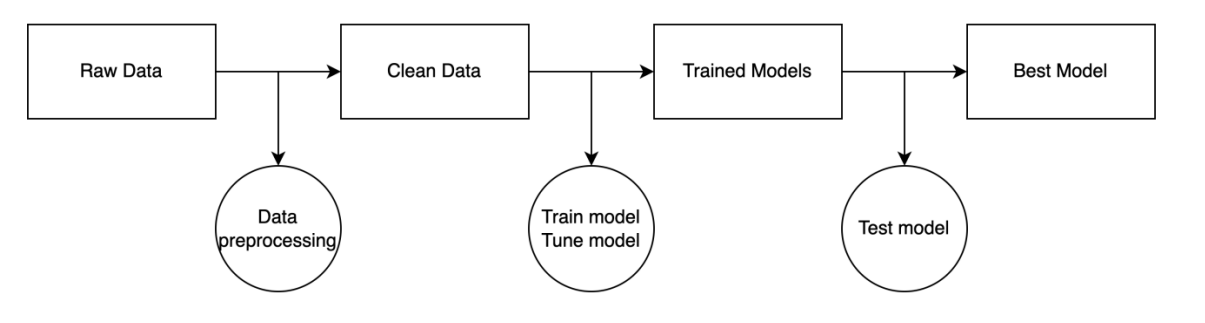
\includegraphics[width=1\linewidth]{quytrinh.png}
    
    
\end{figure}
\end{itemize}
\end{frame}

\section{Tiền xử lý (Data preprocessing)}

\begin{frame}
\frametitle{3. Tiền xử lý (Data preprocessing)}
Quá trình tiền xử lý dữ liệu là bước quan trọng để biến đổi dữ liệu thô trở thành dữ liệu phù hợp cho quá trình huấn luyện của một mô hình AI. Một số quy trình tiền xử lý dữ liệu có thể kể đến bao gồm:
\begin{itemize}
\item Làm sạch dữ liệu (Data cleaning)
\item Tích hợp dữ liệu (Data integration)
\item Thu giảm dữ liệu (Data reduction)
\item Biến đổi dữ liệu (Data transform)
\end{itemize}
Sau khi tiền xử lý, tùy thuộc vào từng bài toán mà ta sẽ chia dữ liệu đã xử lý thành nhiều tập dữ
liệu để sử dụng cho các bước tiếp theo. Một số cách chia thường được sử dụng:
\begin{itemize}
\item Tập huấn luyện (Training sets), tập xác thực (Validation sets) và tập kiểm thử (Test sets)
\item Chia dữ liệu theo thời gian (time series segmentation)
\end{itemize}
\end{frame}

\section{Huấn luyện mô hình (Train model/Tune model)}

\begin{frame}
\frametitle{4. Huấn luyện mô hình}
\begin{itemize}
\item Cách mô hình dự đoán
\item Activation function
\item Loss function
\item Optimizer

\end{itemize}
\end{frame}

\begin{frame}
\frametitle{Cách mô hình dự đoán}
\begin{figure}
    \centering
    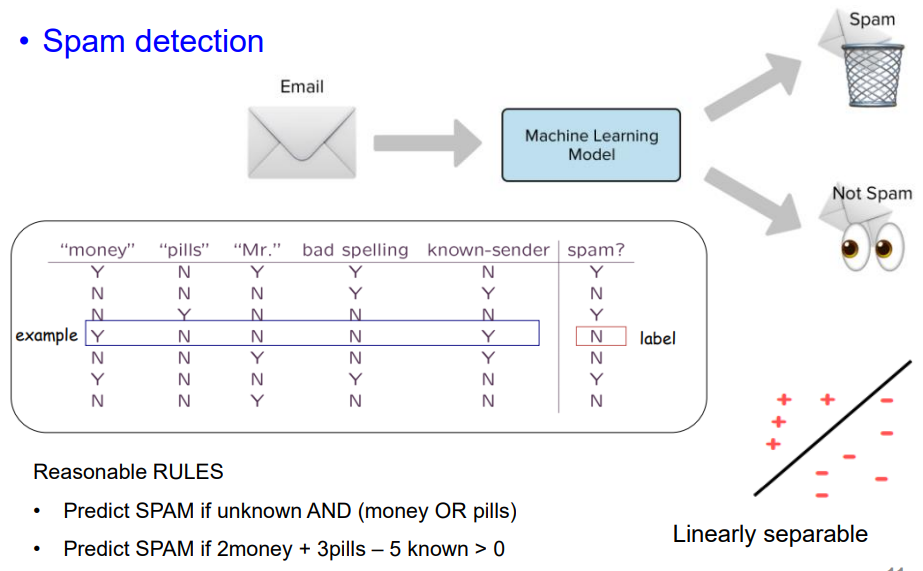
\includegraphics[width=1\linewidth]{predict.png}
    
    
\end{figure}


\end{frame}

\begin{frame}
\frametitle{Activation function}

- \textbf{Hàm kích hoạt} (activation function) của một nút trong mạng neutral nhân tạo là một hàm dùng để tính toán đầu ra của nút đó (dựa trên đầu vào và trọng số của từng đầu vào).
\\- Hàm kích hoạt dùng để xác định đầu ra của mạng neutral. Hàm kích hoạt ánh xạ các giá trị vào khoảng từ 0 đến 1 hoặc -1 đến 1,...(tùy thuộc vào hàm).

\begin{enumerate}
    \item \textbf{Sigmoid (Logistic)}
    \begin{itemize}
        \item 
        \begin{center}
        \large $S(x)=\frac{1}{1+e^{-x}}$
        \end{center}
    \end{itemize}
    
    \item \textbf{Tanh (hyperbolic tangent)}
    \begin{itemize}
        \item 
        \begin{center}
        \large $\tanh x = \frac{e^{x}-e^{-x}}{e^{x}+e^{-x}}$
        \end{center}
    \end{itemize}
    
    \item \textbf{ReLU (Rectified Linear Unit)}
    \begin{itemize}
        \item 
        \begin{center}
        \large $R(x) = max(0,x)$
        \end{center}
    \end{itemize}
    
    \item \textbf{Leaky ReLU}
    \begin{itemize}
        \item 
        \begin{center}
        \large $R(x) = max(0,01x,x)$
        \end{center}
    \end{itemize}
    
\end{enumerate}
\end{frame}

\begin{frame}
\frametitle{Loss function}
\begin{itemize}
    \item Mean Squared Error (MSE)
    \item Mean Absolute Error (MAE)
    \item Cross-Entropy Loss function
\end{itemize}
\begin{figure}
    \centering
    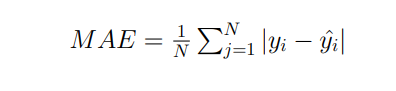
\includegraphics[width=0.7\linewidth]{mae.png}
    
    
\end{figure}
\begin{figure}
    \centering
    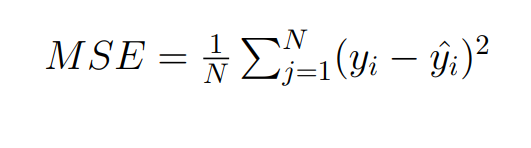
\includegraphics[width=0.7\linewidth]{mse.png}
    
    
\end{figure}

\begin{figure}
    \centering
    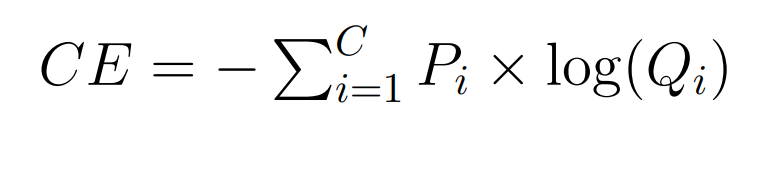
\includegraphics[width=0.7\linewidth]{crosse.png}
    
    
\end{figure}
\end{frame}

\begin{frame}
\frametitle{Optimizer}
\begin{itemize}
    \item Gradient Descent (GD)
    \item Stochastic Gradient Descent (SGD)
    \item Momentum
    \item Adagrad
    \item RMSprop
    \item Adam
\end{itemize}
\end{frame}


\begin{frame}
\frametitle{Optimizer: Gradient Descent}
\begin{figure}
    \centering
    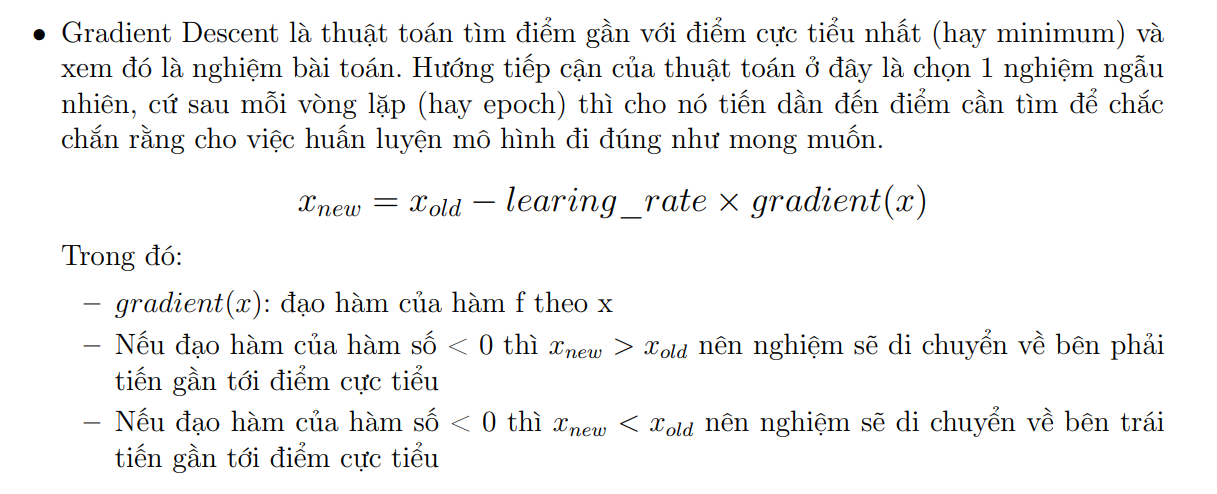
\includegraphics[width=1\linewidth]{gra.png}
    
    
\end{figure}
\end{frame}

\section{Đánh giá mô hình (Test model)}

\begin{frame}
\frametitle{5. Đánh giá mô hình (Test model)}
\begin{itemize}
\item Đo lường hiệu suất để đánh giá mô hình là một phần trong quy trình xây dựng máy học. Tất cả các mô hình máy học đều cần metric để đánh giá hiệu suất
\item Với supervised learning, có 2 bài toán lớn là Regression và Classification. Sau đây là các
metric phổ biến đối với 2 bài toán này:
\begin{itemize}
    \item  Mean Absolute Error (MAE)
    \item Mean Squared Error (MSE)
    \item Root Mean Squared Error (RMSE)
    \item Accuracy
    \item Precision and Recall
    \item F1-score
    \item AU-ROC
\end{itemize}

\end{itemize}
\end{frame}

\begin{frame}
\frametitle{Regression metrics: MAE, MSE, RMSE}
\begin{figure}
    \centering
    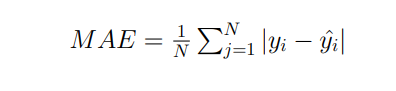
\includegraphics[width=0.75\linewidth]{mae.png}
    
    
\end{figure}
\begin{figure}
    \centering
    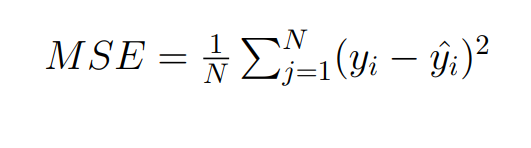
\includegraphics[width=0.75\linewidth]{mse.png}
    
    
\end{figure}
\begin{figure}
    \centering
    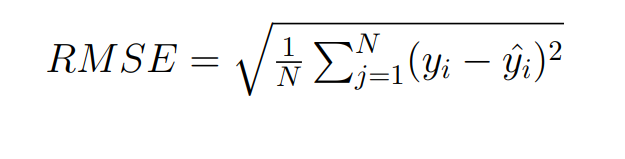
\includegraphics[width=0.75\linewidth]{rmse.png}
    
    
\end{figure}
\end{frame}

\begin{frame}
\frametitle{Confusion matrix: }
\begin{figure}
    \centering
    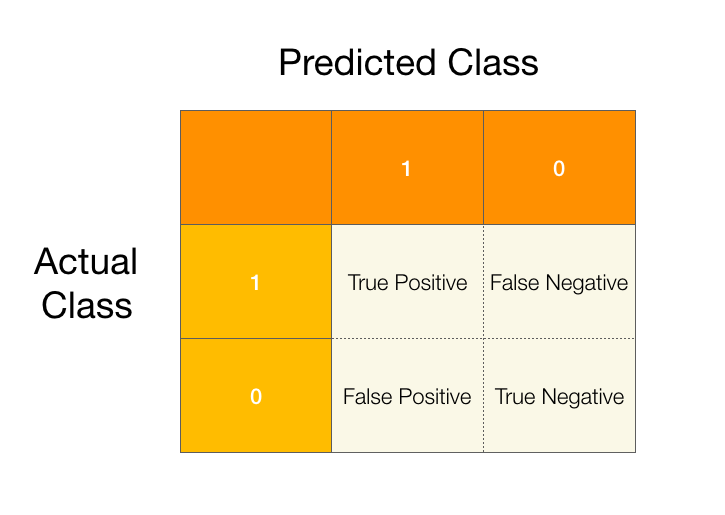
\includegraphics[width=1\linewidth]{cmatrix.png}
    
    
\end{figure}
\end{frame}

\begin{frame}
\frametitle{Classification metrics: Accuracy, Precision and Recall, F1-score, AU-ROC}
\begin{figure}
    \centering
    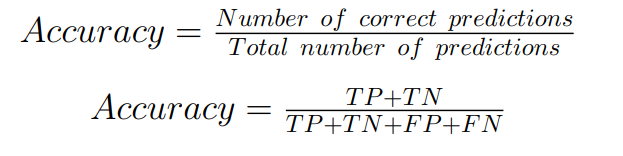
\includegraphics[width=0.6\linewidth]{acc.png}
    
    
\end{figure}
\begin{figure}
    \centering
    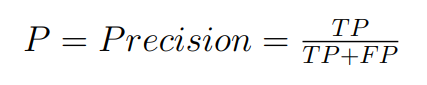
\includegraphics[width=0.5\linewidth]{p.png}
    
    
\end{figure}
\begin{figure}
    \centering
    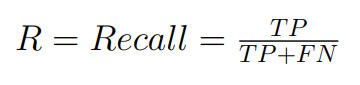
\includegraphics[width=0.5\linewidth]{r.png}

\end{figure}

\begin{figure}
    \centering
    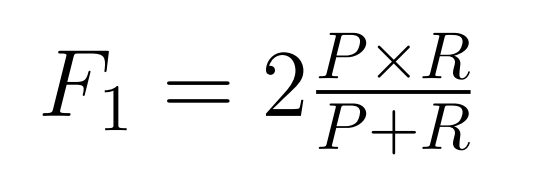
\includegraphics[width=0.35\linewidth]{f1.png}
    
    
\end{figure}

\end{frame}



\begin{frame}
\frametitle{Classification metrics: Accuracy, Precision and Recall, F1-score, AU-ROC}

\begin{figure}
        \centering
        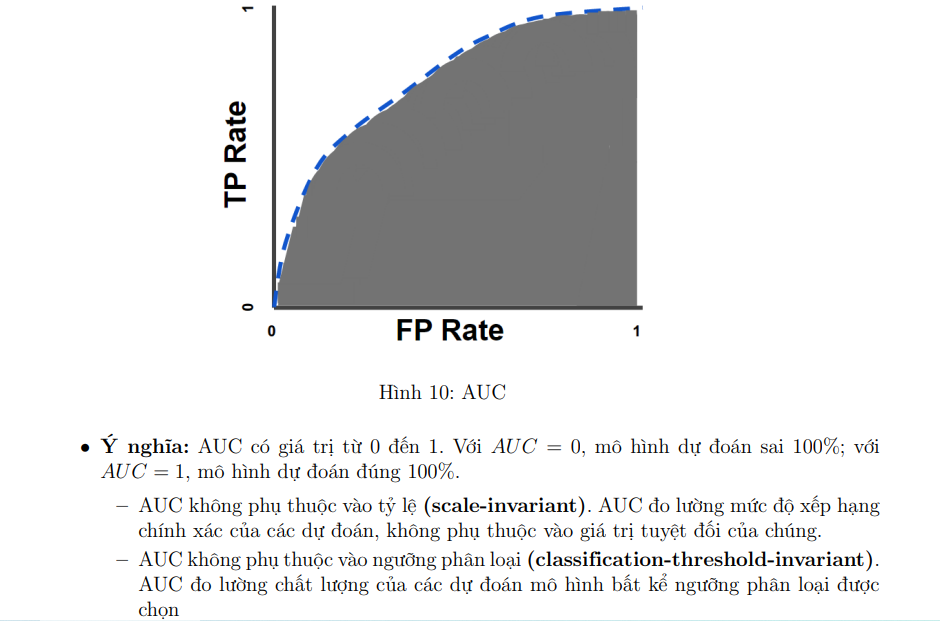
\includegraphics[width=0.75\linewidth]{auc.png}
        
        
    \end{figure}
\end{frame}




\begin{frame}
\Huge{\centerline{The End}}
\end{frame}

%----------------------------------------------------------------------------------------

\end{document} 